Wireless Sensor Nodes \footnote{We will refer instead of the long form to the abbreviation \textsc{WSN} in the remaining documentation.}
are versatile low-power embedded systems used for monitoring sensors, measuring concentration of various chemicals, meshed communication
and a multitude of other purposes.

They were developed by the DARPA\cite{Song}. First tries to establish small networked sensors can be traced back to the cold war according to
\cite{Chong}:

\begin{quote}
    ``During the Cold War, the Sound Surveillance System
    (SOSUS), a system of acoustic sensors (hydrophones) on the
    ocean bottom, was deployed at strategic locations to detect
    and track quiet Soviet submarines. Over the years, other
    more sophisticated acoustic networks have been developed
    for submarine surveillance. SOSUS is now used by the
    National Oceanographic and Atmospheric Administration
    (NOAA) for monitoring events in the ocean, e.g., seismic
    and animal activity.''
\end{quote}

Acconding to Chong et. al the research and development further increased in the year 1980 with the \textsc{Dsn}\footnote{Distributed Sensor Networks} project.
It was founded by the American military while 
``the Arpanet (predecessor of the Internet) had been operational for a number of years, with 
about 200 hosts at universities and research institutes''\cite{Chong}.
R. Kahn, one of the main responsible persons behind the early Internet and co-inventor of the TCP/IP-definitions, had special interest how networked
sensor networks would fit into the routed packed based network acconding to Chong et al..

\begin{figure}[H]
   \centering
   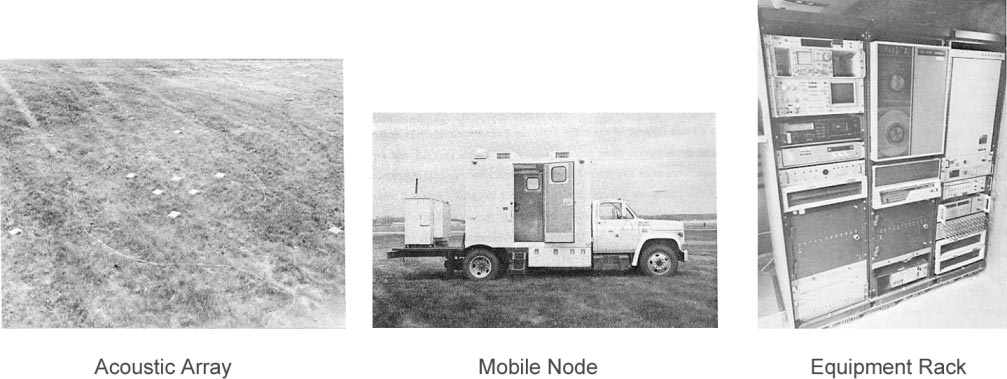
\includegraphics[width=0.8\textwidth]{pic/earlynode.png}%
   \caption{Early Sensor Nodes in 1985. Source: \cite{Chong}}
   \label{earlynode}%
\end{figure}

In~\cite{Akyildiz02wirelesssensor} various applications for military use are described. Main points are:

\begin{description}
    \item[Monitoring] How much ammunition is left in specific areas and/or assets?
    \item[Surveillance] How is the enemy advancing/retreating?
    \item[Reconnaissance] Is in a specific area an opposing force?
    \item[Targeting] Can rockets and other ammunition be assisted for targeting?
    \item[Damage Assessment] How much did our forces suffer before and after a fight?
    \item[ABC Detection] Did the opposing force utilize ABC\footnote{Atom/Nuclear, Biological and Chemical Warfare} weaponry?
\end{description}

As Akyildiz et al. described the main purpose in miliary use are 
``Wireless sensor networks can be an integral part
of military command, control, communications,
computing, intelligence, surveillance, reconnaissance
and targeting (C4ISRT) systems.
''

But rapidly civilian areas of usage were aquired. Heraklit said: ``\gdir{Πόλεμος πάντων μὲν πατήρ ἐστι}''\footnote{War is the father of all things} and so 
research and development about wireless sensor networks was adapted by universities and other parties.

The main points which stopped the usage in civilian areas were:

\begin{itemize}
\item battery longlivety
\item size
\item portability
\item secure communication
\item calculation speed
\item compatibility
\item lacking unified language for high-level programming
\end{itemize}

If one \textsc{WSN} is not enough for a usage scenario some form of communication between the devices is neccessary. The obvious
route is through means of wireless communication.

Different forms of wireless communication are available:

\begin{description}
\item[ZigBee] Low power but limited range
\item[IEEE 802.11] Popular name is \textsc{WLAN}. Mainly the 2.4 GHz band is used but in subsets like 802.11a the short-waved 5GHz band is usable.
Energy consumption is generally higher.\footnote{Regulatory standards in Germany forbid more than 150mA total power sent.}
\item[ANT+] A whole stack which focuses on low-power embedded applicances
\item[LPD433] Low-power band around 433 MHz used for custom communication for devices. Also low range albeit low power.
\end{description}

Nodes use various, multiple or even cable bound means of communication. A common problem is the intercommunication between devices for 
exchanging data. Even if the nodes in a project are plain reporting devices with no input command interface the possiblity for
querying the reported data with external devices as handhelds, smartphones, tables or other mobile devices could open new possibilites.

Web language queries via the http protocol are favourable due to less limitations on different firewalls and NAT\footnote{Network Address Translation is a
method for using public IPv4 addresses for multiple end devices.}  restrictions. Figure~\ref{fig:problem} shows an example where the microwave cannot
be controlled by a mobile device or other possible scenarios.\footnote{Note that more useful things are also planned as a possibility to check for 
temperatures in various node supplied data centers which are queried by the technician over his mobile - push-service as it gets too hot.
\gdir{οἱ πολλοί} will fastly adapt it even without knowing they use it.}

\begin{figure}[h]
   \centering
   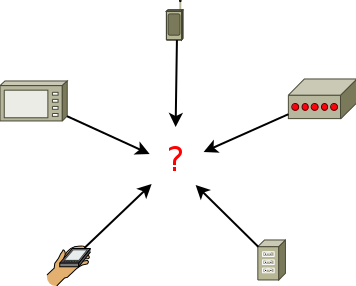
\includegraphics[width=0.4\textwidth]{pic/problem.png}%
   \caption{Different Embedded Devices use Various Languages}
   \label{fig:problem}%
\end{figure}


Wireless sensor nodes can be deployed and used in a multitude of means.\footnote{But not for special cases as~\cite{biederbeck}}
